\documentclass{standalone}
\usepackage{tikz}
\usepackage{pgfplots}
\pgfplotsset{compat=1.16}
\begin{document}
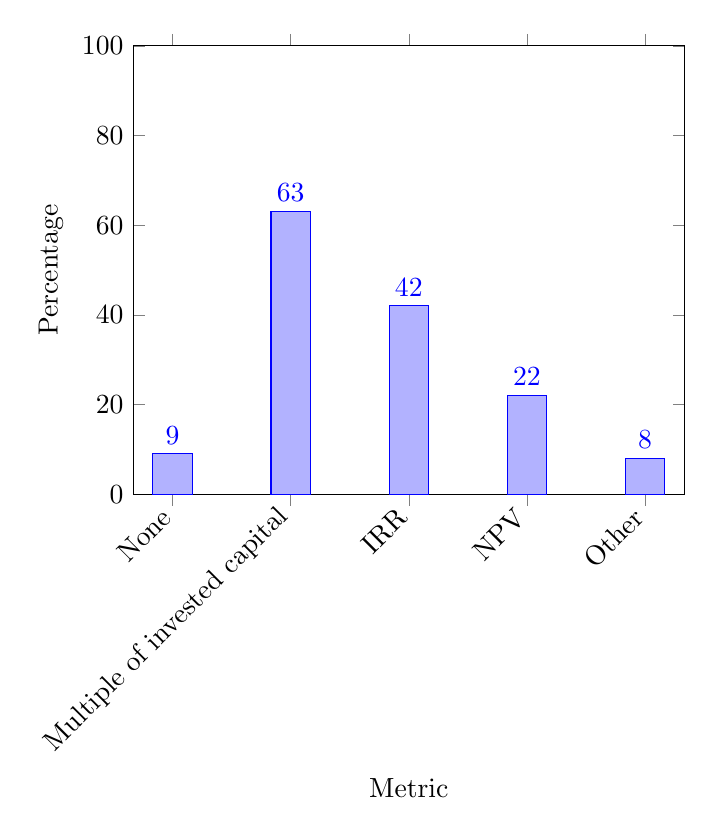
\begin{tikzpicture}
\begin{axis}[
ybar,
bar width=0.5cm,
x=1.5cm,
enlarge x limits={abs=0.5cm},
symbolic x coords={None, Multiple of invested capital, IRR, NPV, Other},
xtick=data,
nodes near coords,
nodes near coords align={vertical},
ymin=0,
ymax=100,
ylabel={Percentage},
xlabel={Metric},
x tick label style={rotate=45, anchor=east},
]
\addplot coordinates {
(None, 9)
(Multiple of invested capital, 63)
(IRR, 42)
(NPV, 22)
(Other, 8)
};
\end{axis}
\end{tikzpicture}
\end{document}